\documentclass[12pt]{report}
\linespread{2}
\usepackage[pdftex]{graphicx}   
\usepackage{amssymb}
\usepackage{tocbibind}
\usepackage[utf8]{inputenc}
\usepackage[english]{babel}
\usepackage{natbib}
\usepackage{amsmath}
\usepackage{multirow}
\usepackage{graphicx}
\usepackage{stackengine}
\usepackage{subcaption}
\usepackage[margin=1.25in]{geometry}
\usepackage[nodayofweek]{datetime}
\newdateformat{mydate}{{ }\shortmonthname[\THEMONTH], \THEYEAR}

\newdateformat{myyear}{{ }\THEYEAR}
% latex
% \usepackage[hidelinks]{hyperref}
\usepackage{hyperref}
\usepackage[hyphenbreaks]{breakurl}

\usepackage{booktabs}
%\usepackage{lineno}
%\linenumbers
\usepackage{calc}  
\usepackage{enumitem}  
%\usepackage{sectsty}
%
%%\chapternumberfont{\tiny} 
%\chaptertitlefont{\huge}

%opening
\title{Improving Neural Machine Translation for Morphologically rich languages }
\author{Raja Gunasekaran}

\usepackage{graphicx}
\usepackage{pdfpages}
\graphicspath{ {images/} }

\begin{document}


\pagenumbering{roman}
%\thispagestyle{empty} %remove page number from title page
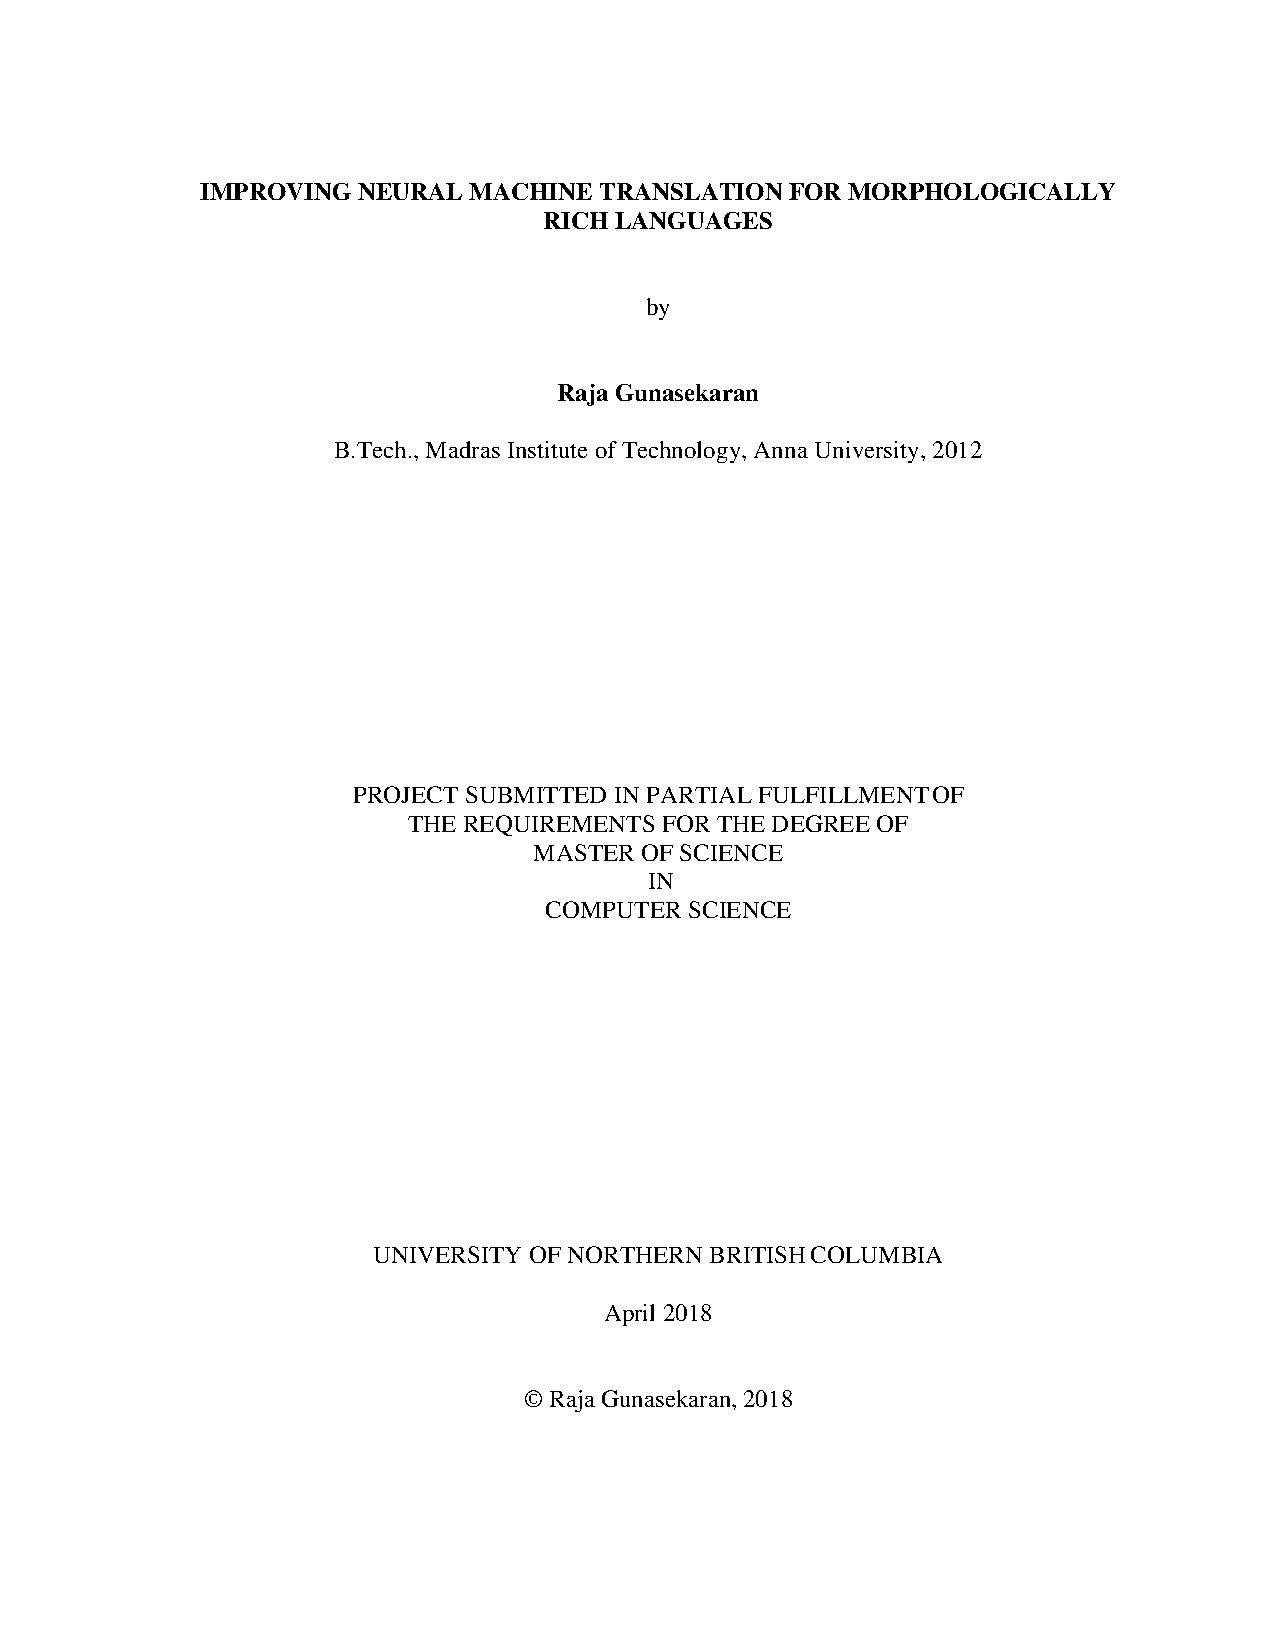
\includepdf{tex/title.pdf}
	
%\setcounter{page}{2} % Title Page gets number "i"
%\thispagestyle{empty} %remove page number from title page	
%\pagenumbering{roman}
\thispagestyle{empty}
\topmargin 0in

\vspace*{.3cm}
\begin{center}
\begin{large} 
\textbf{Improving Neural Machine Translation For Morphologically Rich Languages}
\end{large}

\vspace*{.6cm}

by

\vspace*{.6cm}

\textbf{Raja Gunasekaran}

B.Tech., Madras Institute of Technology, Anna University, 2012\\


\vspace*{4cm}

PROJECT SUBMITTED IN PARTIAL FULFILLMENT OF\\
THE REQUIREMENTS FOR THE DEGREE OF\\
MASTER OF SCIENCE\\
IN\\
COMPUTER SCIENCE\\
 
\vspace*{4.5cm}

UNIVERSITY OF NORTHERN BRITISH COLUMBIA\\
   
\vspace*{.002cm}
   
\mydate
\today

\vspace*{.25cm}

\copyright  Raja Gunasekaran, \myyear
\today
\end{center}



\pagestyle{plain}
\clearpage
\begin{center}
	\textbf{Abstract}
\end{center} 

Machine Translation aims to provide a seamless communication and interaction,  thereby overcoming human language barriers. Recently, Neural Machine Translation (NMT) approaches have been very successful and achieve state-of-the-art performance in many language pairs. NMT systems consist of millions of neurons that are optimised to learn the input-output mapping between the source and the target languages. However, these systems produce poor translation quality under low-resource conditions and are unable to handle a large vocabulary particularly for languages with rich morphology such as Turkish, Tamil and German.

In this project, we present a source vocabulary expansion technique to handle the problem of translating rare and unknown words by incorporating morphological information in the words. The effectiveness of the proposed technique is demonstrated by translating from two morphologically rich languages to English. Using this technique, we achieve a performance gain of approximately 2 BLEU points for both German $\rightarrow$ English and Turkish $\rightarrow$ English. 
\phantomsection\addcontentsline{toc}{chapter}{Abstract}
\tableofcontents
\listoftables
\listoffigures
\newpage
\pagenumbering{arabic}


%\addcontentsline{toc}{chapter}{\abstractname}
%\begin{abstract}	
%\end{abstract}
%\cleardoublepage
%\listoffigures
%\cleardoublepage
%\addcontentsline{toc}{chapter}{\listfigurename}
%\listoftables
%\cleardoublepage
%\addcontentsline{toc}{chapter}{\listtablename}

\chapter{Introduction}
%\section{Introduction}

%NMT systems are well suited for any problem that can be formulated as mapping an input sequence to an output sequence \citep{sutskever2014sequence}.
Human languages are very diverse and are different from each other in many aspects. There are around 6000 - 8000 languages that are currently spoken in the world. This count varies based on the definition of a \textit{language} \citep{evans2009myth}. This diversity also creates a barrier in communication and interaction. Machine Translation is a promising field that can be used to overcome the human language barrier. With the recent technological advancements in communication, there is an increasing need for seamless communication and content assimilation across languages. 

Machine Translation (MT) is the process of translating text automatically from one natural language to another \citep{russell2002artificial}. The development of MT systems can be broadly classified into three: rule based approach, statistical approach, and neural network based approach. Starting from the 1980s until recently, Statistical Machine Translation (SMT) approaches like phrase-based translation models \citep{och2002statistical,koehn2003statistical} gave promising results and dominated the field of machine translation. They were widely adopted and used in most of the translation engines. 


Neural Machine Translation (NMT) is a recent approach to MT using neural networks.  \cite{kalchbrenner2013recurrent} proposed the first, successful end-to-end system using encoder-decoder architecture for MT. This led to rapid development of more complex encoder-decoder models by \cite{sutskever2014sequence,cho2014learning,bahdanau2014neural,vaswani2017attention}, each with additional functionality and improved performance. In the \textit{Conference on Machine Translation (WMT 2015)}, only one purely neural network based MT system was submitted, and it was outperformed by a statistical MT system. In the 2017 WMT conference, almost all the systems were NMT systems \citep{koehn2017neural}. As a result of this rapid development, popular translation engines like Google NMT, Microsoft Translator and Systran adopted NMT as a base technology for their translation system.

NMT requires a parallel corpus of source language and target language sentence pairs. These systems 
%, like other neural NLP systems, 
learn vector representation of the input words called \textit{word embeddings}. It is a way of representing words in a language using \textit{d-}dimensional \textit{word vector} $\vec{w} \in \mathbb{R}^{d}$. The word vectors capture essential information about the words such as semantics and morphology. In word vectors generated using continous bag of words(CBOW) models, a simple arithmetic on them can be used to answer analogies like \textit{man is to king as woman is to X} as shown below. 

\begin{align*}
\vec{man} - \vec{woman} + \vec{king} &  \approx \vec{queen} \\
\vec{walking} - \vec{walk} + \vec{stop} & \approx \vec{stopping}
\end{align*}



NMT systems will use the information captured in the word vectors and learn an input-output mapping, from a source language to the target language. The word vectors from the input sequence passed into a neural network are first mapped to a fixed length vector as shown in Figure \ref{enc_dec}. From this fixed length vector, the target language sentence is generated word by word. As words occur more often, they get semantically more accurate vector representations and are translated more accurately. %than the words that occur only a few times. 
Because of this, NMT requires a large training dataset to learn the mapping from an input (source) language to the output (target) language. 


\begin{figure}[ht]
	\centering
	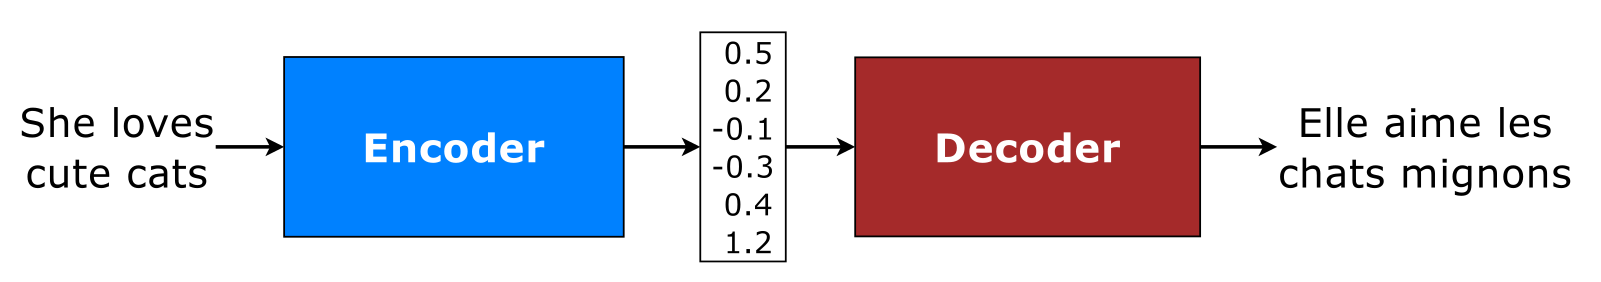
\includegraphics[scale=0.27]{images/enc_dec}
	\caption{General architecture of NMT systems. Figure taken from \cite{luong2016neural}}
	\label{enc_dec}
\end{figure}
%Because of this, common words are translated more accurately than rare and unknown words.

\section{Motivation}
%For example, these systems do not perform well  Another major challenge in NMT systems is their inability to handle large vocabulary\citep{koehn2017six}. 
Although NMT systems have shown promising results in the past few years, there are a number of challenges that these systems face. Some of the major challenges are: poor translation quality under low-resource conditions, poor translation of out-of-domain data, and inability to handle a large vocabulary \citep{koehn2017six}. These challenges are usually more pronounced in languages with rich morphology. 

\subsection{Morphologically rich, low-resource languages}
Morphologically rich languages such as Turkish, Tamil, German, Finnish etc., encode more information like gender, tense, number, etc. in a word as shown in Table \ref{turkish}. These languages also have a very large vocabulary since there can be large number of word forms per lexeme. Morphologically poor languages like English rely on word order (syntax) and context to convey this information. %In English, \textit{run, running, ran, runs} are all the forms of same lexeme \textit{run}.



\begin{table}[ht]
	\centering
	\resizebox{!}{4cm}{
	\begin{tabular}{@{}ll@{}}
		\toprule
		\textbf{Turkish}             & \textbf{English}                             \\ \midrule
		duy(-mak)                   & \textit{(to) sense}                          \\
		duygu                       & \textit{sensation}                           \\
		duygusal                    & \textit{sensitive}                           \\
		duygusallaş(-mak)           & \textit{(to) become sensitive}               \\
		duygusallaştırılmış         & \textit{the one who has been made sensitive} \\ 
		duygusallaştırılamamış      & \textit{the one who could not have been made sensitive} \\		
%		duygusallaştırılamamışlardan & \textit{from the ones who could not have been made sensitive} \\ \bottomrule
	\end{tabular}}
	\caption{Turkish - English Translation \citep{ataman2017linguistically} }
	\label{turkish}
\end{table}

Although benefits of NMT have been realized in high resource languages such as English and French, NMT is still a poor choice for languages, where parallel data for training is scarce. Neural methods learn poorly from low amount of data and hence, require a lot of data to perform well. 

\subsection{Research Problem}

The primary focus of this project is to improve the quality of machine translation for morphologically rich languages under low resource settings. NMT systems use a limited vocabulary, from 30,000 to 80,000 words, to control the computational complexity during training. While this vocabulary size is  large enough for languages like English, the performance of these models suffer in morphologically rich languages. To overcome this,  \cite{sennrich2015neural} proposed a system that can reduce the vocabulary size by splitting the words into common subwords. While this approach is sometimes sufficient, the words are not split at morphological boundaries.

Many inflected forms of words, as shown in Table \ref{turkish}, are usually scarce in the training dataset. Hence, the semantic and morphological information in the words is not captured in their word vectors. Addressing this problem can help us to improve the quality of machine translation for low-resource, morphologically rich languages.


In this project, we present a source language vocabulary expansion technique for handling a large vocabulary in NMT. This technique is particularly useful for low-resource, morphologically rich languages. The vocabulary is expanded based on morphological analysis of the Out of Vocabulary (OOV) words. For this purpose, we use a word embedding model based on sub-word units from \cite{bojanowski2016enriching}. To demonstrate the effectiveness of this approach, we present experimental evaluations on Turkish$\rightarrow$English and German$\rightarrow$English translation task. For comparison, we use global attention based NMT from \cite{luong2015effective} as a baseline.

%These systems are only as good as the data they are trained on. While English represents only 9\% of the world population, 54\% of the digital content is in English.
%This  Embedding models discussed in  \cite{bengio2003neural}, \cite{mikolov2013distributed}, \cite{pennington2014glove}, etc., learn word representations in continuous vector space where similar words occur closer to each other.  To get a good representation for each word the system has to be trained on large dataset of million of sentence. These word vector can also be trained on a large monolingual corpus and reused other tasks like machine learning.

%Another disadvantage of improving the vocabulary size, is that 


%The focus of this project will on the performance of NMT systems under low resource settings for morphologically rich languages.
%
%One of the challenges when using pre-trained word embeddings for any natural language processing (NLP) task is the issue of handling out-of-vocabulary (OOV) words. This problem occurs when a word that was unseen during training time occurs in testing phase during translation.  In this project, I propose and implement an NMT systems based on \cite{bahdanau2014neural} that is able to handle OOV words online during translation. OOV words will be analysed for their morphology and mapped to an in-vocabulary word using the technique from \cite{soricut2015unsupervised}.


%\subsubsection{Report outline}

\section{Report outline}

The project report is organized as follows. Chapter \ref{background} gives a background on recurrent neural networks and historical approaches for machine translation. In Chapter \ref{related}, related NMT systems that handle unknown words and their techniques are presented. In Chapter \ref{proposed}, we discuss our proposed vocabulary expansion technique and its architecture in detail. In Chapter \ref{comparision1}, we report on our comparison study of different techniques to handle OOV words. In Chapter \ref{experiments}, we present an evaluation of the proposed work on machine translation tasks for two language pairs. Finally, in Chapter \ref{conclusion}, we conclude the project report and provide future directions to extend the work carried out in this project.

%Dataset used in the project and evaluation metric are presented in Chapter \ref{experiments}. In the last section, the implementation status and timeline for the projects is given.
%
%a classic NMT model from \cite{bahdanau2014neural} and extending the work of \cite{soricut2015unsupervised} for handling OOV words online during translation. 




\chapter{Background}
\label{background}
%\section{Background}
This section provides a background on two main topics of the project: Recurrent Neural Networks (RNN) and Machine Translation (MT). We begin by looking into neural networks and why RNNs are well suited for MT. Then, we will look into some of the historical and current approaches for machine translation.

\section{Neural Networks}
\cite{rojas2013neural} define neural networks as ``distributed, adaptive, generally nonlinear learning  machines built from many different processing elements''. They can approximate a function by learning the input-output mapping. Neural networks like feed-forward multi-layer perceptrons, shown in Figure \ref{mlp}, can approximate any (continuous) function to an arbitrary accuracy if the number of hidden neurons are large enough \citep{hornik1989multilayer}. These networks can be trained using the backpropogation algorithm \citep{rumelhart1988learning} by updating the weights and biases based on an objective function. As the training progresses, the network updates its weights in a way that its predicted output moves closer to the ground truth\footnote{ground truth - reference output provided by direct observation as opposed to inference}. A one layer feed-forward neural network can be written as follows:


%of the network to match the predicted output to the labelled output
\begin{equation}
NN_{MLP1} (x) = g(xW^1 + b^1 )W^2 + b^2
\end{equation}

where g is any non linear activation function, $x$ is an input vector, $W^1, W^2, b^1$ and  $b^2$ are the weights and biases for the network.

Unlike other machine learning approaches where input features have to be hand-engineered, neural networks can learn the required features from the training data. 

\begin{figure}[ht]
	\centering
	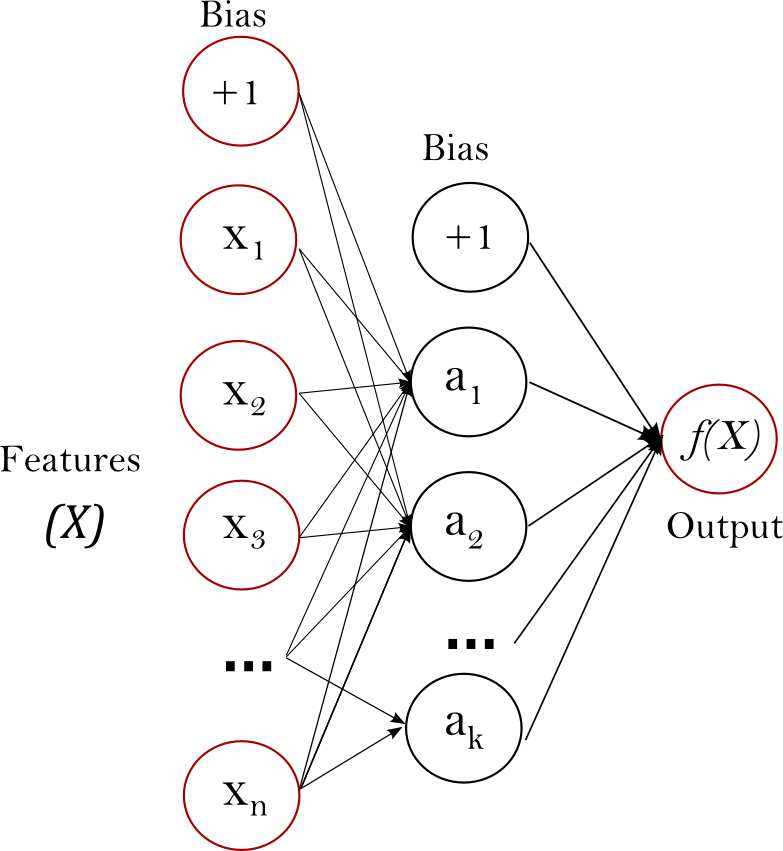
\includegraphics{images/multilayerperceptron_network}
	\caption{Multilayer perceptron network with one hidden layer. Figure taken from  \cite{pedregosa2011scikit}}
	\label{mlp}.
\end{figure}

One class of neural network model called Recurrent Nerual Network (RNN) \citep{elman1990finding} is particularly well suited for machine translation. In natural languages, the input is a sequence of words of arbitrary length based on some structure properties of the language. RNNs allow for representing an input sequence of arbitrary length as fixed-sized vectors based on its structural properties. A simple RNN \citep{goldberg2016primer} can be defined as follows.

\begin{align}
h_{1:n},  y_{1:n} &= RNN(h_0,x_{1:n}) \\
h_i &= R(h_{i-1},x_i;\theta) \\
y_i &= O(h_i;\theta)
\end{align}
\[ 
x_i \in \mathbb{R}^{d_{in}}, y_i \in \mathbb{R}^{d_{out}}, h_i \in \mathbb{R}^{f({d_{out}})} \]

where $x_{1:n}$ is the input vector, $y_{1:n}$ is the output vector and $h_{i}$ is the state vector at time-step $i$. $R$ is a non linear function applied over current input $x_i$ and previous hidden state $s_{i-1}$. $O$ is an additional function applied over the current hidden state to generate output vector.  Parameters $\theta$ are shared across the network. A simple RNN uses $sigmoid$ or $tanh$ as the non linear function in the neural units. Special kinds of neural units like Long Short-Term Memory (LSTM) \citep{hochreiter1997long} or Gated Recurrent Units (GRU) \citep{cho2014learning} can also be used. A graphical representation of the same network is shown in Figure \ref{rnn}


\begin{figure}[ht]
	\centering
	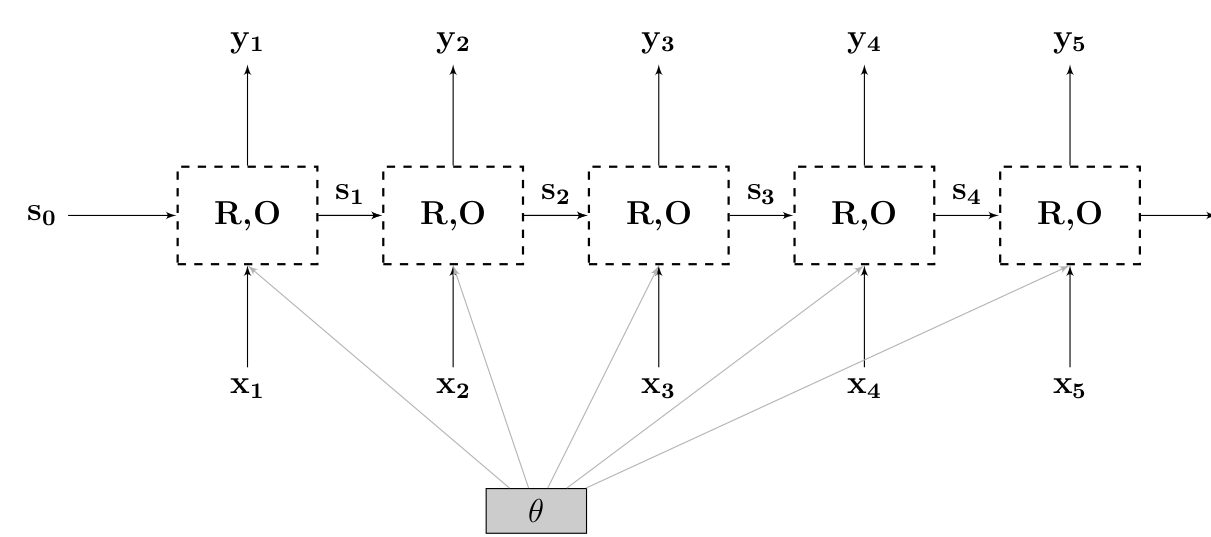
\includegraphics[scale=0.3]{images/rnn}
	\caption{Graphical representation of RNN. Figure taken from \cite{goldberg2016primer}}.
	\label{rnn}
\end{figure}


The input for these neural networks is a sequence of vectors not words. NMT systems use word embeddings to represent input words. It is a way of representing words in a vocabulary as vectors in a higher dimensional space. These representations have been good at capturing semantic and syntactic regularities in languages \citep{mikolov2013distributed}. When used as input, these models have also been shown to improve the performance of many NLP systems in tasks such as \textit{MT} \citep{vaswani2017attention, sennrich2015neural}, \textit{sentiment classification} \citep{kumar2016ask}, and \textit{part of speech tagging} \citep{kumar2016ask}. The vector representation for words in these models primarily depend their co-occurrence count with other words within a window size. These vectors capture syntactic, semantic and morphological properties of the words. 

%\begin{figure}[ht]
%	\centering
%	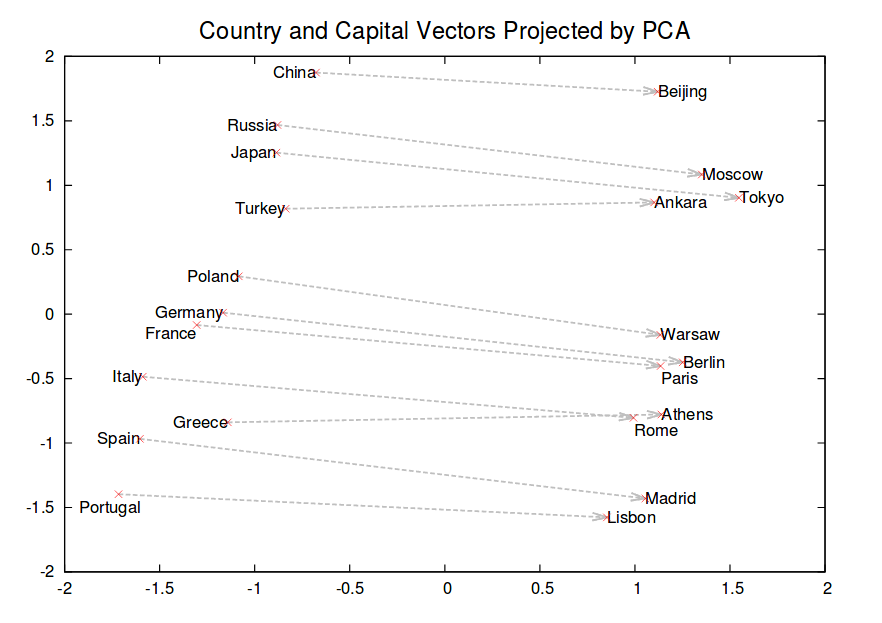
\includegraphics[scale=0.5]{images/embeddings}
%	\caption{Two-dimensional Principal component analysis (PCA) projection of 1000-dimensional vectors of countries and their capitals \citep{mikolov2013distributed}}.
%	\label{embeddings}
%\end{figure}


%\footnote{Principal component analysis (PCA is dimensionality technique used here to show high dimensional vectors in 2-dimensional space.)}

One of the major challenges for many embedding models is their inability to handle Out Of Vocabulary (OOV) words.  This problem is more pronounced in languages with rich morphology. A word in morphologically rich languages encodes more information (such as gender, number, tense) as compared to morphologically poor languages which rely on word order and context. Recently, many models have been proposed to solve this problem. \cite{sun2016inside} proposed a method to integrate both external contexts and internal morphemes\footnote{Morphemes are the smallest meaningful units in a language.} to learn better word embeddings especially for rare and unknown words. \cite{bojanowski2016enriching} incorporate subword information like character n-grams\footnote{A character n-gram is a sequence of n characters from a word} for learning word embeddings during training. Overall, character embedding models, where vector representations for every character or character n-grams are learned, have be shown to generate good word embeddings for rare and unknown words. 

%%Most of these models were originally developed in English - a language with strict word order and relatively poor morphology. These models perform the best in English. 
%

%
%
%Despite their advantages, NMT systems are not capable of translating rare and unknown words. In this project, I am implementing an end to end encoder-decoder system for machine translation and an unsupervised method to handle unknown and rare words.
%

\section{Statistical Machine Translation}
Machine translation is a task of translating a source language sentence $F$ to the target language sentence $E$ using computing resources. It can effectively remove language barriers between humans, allowing assimilation of content from different languages. This potential of MT has led to substantial amount of research since the advent of digital computing. There have been many approaches to the problem such as rule-based MT, phrase-based MT, NMT, etc. In the early days, rule based approaches that used dictionaries, grammar and pre-defined rules to translate text were explored until the ALPAC report in 1966 \citep{national1966language}. The ALPAC report showed that post-editing machine translation was not cheaper or faster than human translation. 

%\subsubsection{Statistical Machine Translation}

In the late 1980s, following the success of statistical method on speech recognition, IBM research \citep{brown1993mathematics} modelled the problem of translation as a statistical optimization problem. Many SMT approaches such as word-based models \citep{brown1993mathematics}, phrase-based models \citep{koehn2003statistical,marcu2002phrase}, hierarchical phrase-based  models \citep{chiang2007hierarchical} and syntax based models \cite{galley2004s,galley2006scalable} were proposed. The goal of all the SMT systems is to maximize the probability of target sentence $f$ given the source language sentence $e$

\begin{equation}
\underset{f}{argmax \  } P(f|e) = \underset{f}{arg max } (P(f) \times P(e|f)) 
\end{equation}


where $P(f)$ is a language model and $P(e|f)$ is a translation model. Language model and translation model are sub-components of SMT systems. Language models learn to assign probability to a sequence of words in a language. They assign higher probability to sentences that are more likely to occur in the language and hence a measure of fluency in the language. Language modelling is central to many tasks in NLP including MT.  

Translation models learn the mapping between source and target language words or phrases. They measure word level translation accuracy between source and target sentences. These models were built by analyzing  monolingual, bilingual corpus and learning their probability distribution. The rise of digital text resources like parallel corpora and an increase in computing power and storage, fuelled the growth of SMT systems. Although SMT systems are robust to noisy data,  they required fine tuning for many components such as language model, reordering model, and translation model for each language pairs. They also require large amount of data and do not handle long range dependencies well.


\section{Neural Machine Translation}

An NMT system is a neural network that models the conditional probability $p(y|x)$ of generating a target language $y$ sentence given the source language sentence $x$. Generally, any NMT system consists of two components i) an \textit{encoder} that computes a sentence representation vector from the source sentence, and ii) a \textit{decoder} that transforms the vector representation to a target language sentence. RNNs are a common choice of network for both encoders and decoders as they process input in a sequential fashion. Convolution neural networks have also been used especially as an encoder \citep{kalchbrenner2013recurrent}.

%In 2003, \cite{bengio2003neural} proposed probabilistic language model based on neural networks which laid the foundation for the use of neural networks in machine translation. 

Initially, neural networks were used as a component in phrase based systems to score the quality of translation \citep{schwenk2012continuous} and to provide additional features to SMT systems \citep{zou2013bilingual}. \cite{kalchbrenner2013recurrent} proposed the first end to end approach for NMT using convolution neural networks as the encoder and RNN as the decoder. Their network suffered from the problem of vanishing gradients where the network was unable to capture long range dependencies. To overcome this problem, more sophisticated activation functions such as LSTM \citep{hochreiter1997long} or GRU \citep{cho2014learning} are used.  \cite{sutskever2014sequence} and \cite{cho2014learning} demonstrated that these gated units can handle long range dependencies better than a simple RNN \citep{elman1990finding}. An encoder-decoder network with LSTM RNNs is shown in Figure \ref{seq2seq}. The boxes in the figure are LSTM RNN units. Mathematically, an LSTM RNN unit is defined in \cite{goldberg2016primer} as follows:

\begin{align}
s_j = R_{LSTM}(s_{j-1}, x_j) &= [c_j:h_j] \\
c_j &= c_{j-1} \odot f + g \odot i \\
h_j &= tanh(c_j) \odot o \\
i &= \sigma(x_j W^{xi} + h_{j-1} W^{hi})\\
f &= \sigma(x_j W^{xf} + h_{j-1} W^{hf})\\
o &= \sigma(x_j W^{xo} + h_{j-1} W^{ho})\\
g &= tanh(x_j W^{xg} + h_{j-1}W^{hg})\\
y_j &= O_{LSTM}(s_j)
\end{align}
\[ 
s_i \in \mathbb{R}^{2 \cdot d_{h}}, x_i \in \mathbb{R}^{d_{x}}, [c_j, h_j, i, f, o, g] \in \mathbb{R}^{{d_{h}}}, W^{xo} \in \mathbb{R}^{d_x x d_h}, W^{ho} \in \mathbb{R}^{d_h x d_h}  \]

where $x_j$, $y_j$ and $h_j$ are the input vector, output vector and the hidden vector repectively. $\odot$ is component-wise product. $i$, $f$ and $o$ are input, forget and output gates respectively. $g$ is the update candidate.

\begin{figure}[ht]
	\centering
	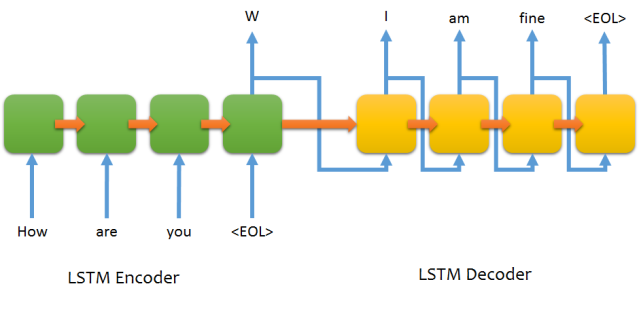
\includegraphics[scale=0.9]{images/seq2seq}
	\caption{RNN with LSTM encoder and decoder. Figure taken from \cite{farizrahman4u}}.
	\label{seq2seq}
\end{figure}


\subsubsection{Attention based Encoder-Decoder models}

These simple encoder-decoder networks summarize the source sentence in a fixed length context vector. \cite{bahdanau2014neural} noted that these networks were inadequate to represent long sentences due to the fixed dimension of the context vector. While this problem could theoretically be solved by increasing the dimension of the context vector, the computing power and memory required to train such a network sets an upper limit even today.

\cite{bahdanau2014neural} proposed an attention based encoder-decoder architecture to mitigate this problem.  This allowed for the encoder to produce better sentence representation for longer sentences which in turn improved the translation quality. In their additive approach, a single feed forward neural networks that can learn to assign different weights to the hidden layer vectors was used. These weighted sum of the hidden layer vectors $h_{1:n}$ called context vector $c_i$ is calculated each time decoder generates a new word as shown in Figure \ref{attention}.

\begin{align}
c_i &= \sum_{j=1}^{n} \alpha_{ij} h_j \\
\alpha_{ij} &= \frac{\hat{a}_{ij}}{\sum_j \hat{a}_{ij}}\\
\hat{a}_{ij} &= att(s_i, h_j)
\end{align}


%\cite{bahdanau2014neural} proposed an attention based encoder-decoder architecture which is capable of learning word alignment between source and target sentences.In their additive approach, a single feed forward neural networks that can learn to assign different weights to the hidden layer vectors was used. 


where $att(s_i, h_j)$ is an attention function that calculates the weights for each encoder hidden state $h_{1:n}$, for a given decoder state $s_i$. They also used bi-directional RNN which reads the sentence from both directions. The state vector from both direction right to left  $\overleftarrow{h_j}$ and left to right $\overrightarrow{h_j}$ is concatenated for each word. The attention mechanism is applied over this concatenated hidden state vector $h_j = [\overleftarrow{h_j};\overrightarrow{h_j}]$. The whole network is trained with negative log-likelihood as the objective function using stochastic gradient descent.


\begin{figure}[ht]
	\centering
	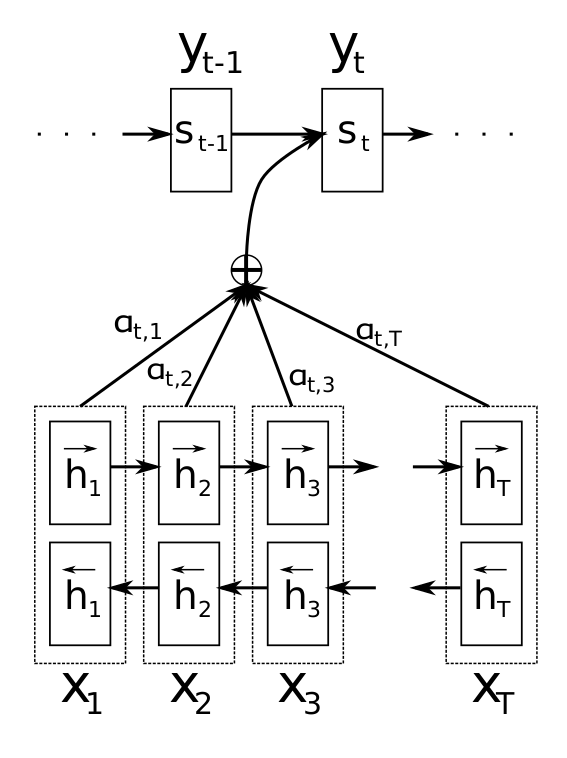
\includegraphics[scale=0.35]{images/attention}
	\caption{Attention based encoder. Figure taken from \cite{bahdanau2014neural}}.
	\label{attention}
\end{figure}


%\begin{align}
%a_t(s) = align(h_t, \bar h_s)  = \dfrac{exp(score(h_t, \bar h_s))}{\sum_{s'} exp(score(h_t, \bar h_{s'}))}
%\end{align}

\cite{luong2015effective} proposed two simpler but effective variations of attention mechanism namely: 1) a global attention model where all words in the source sentence are attended, and 2) a local attention model where only a subset of the source words are attended at a time. In the global attention mechanism, which is very similar to one proposed in \cite{bahdanau2014neural}, they did away with bi-directional, concatenated state vector $h_j = [\overleftarrow{h_j};\overrightarrow{h_j}]$. They simplified the computation path to make it run faster. Their model produced state-of-the-art results in WMT'14 and WMT'15 for English to German translation. 


In this project, we use the global attention based encoder-decoder model proposed in \cite{luong2015effective} as the baseline NMT system for evaluation. The models discussed so far cannot handle words that are not in their vocabulary. In the next chapter, we will look at some of techniques that allow us to handle OOV words.




% Basics needed to understand the rest of the text with references to authoritative literature sources

%
%
%
%
%In their model, the source language sentence will be encoded into a real valued vector using the encoder. The decoder will decode the vector to a target language sentence to produce the output. 
%
%Unlike, SMT systems, NMT systems generalize well, do not require domain knowledge and are more tolerant to noisy data \cite{bibid}. 
%
%
%NMT systems use vector representation, also called word embeddings, for input words and internal states. Word embedding is a way of representing words in the vocabulary using vectors in a high dimensional space.Word embedding models like \cite{bengio2003neural,mikolov2013distributed,pennington2014glove} etc., learn word representation in continuous vector space where similar words are expected to occur closer to each other. These models have been successfully used in many NLP tasks like Machine Translation. The vector representation for word in most of these models primarily depend on word co-occurrence or context words within a window size capturing syntactic, semantic and morphological properties of natural languages. 
%
%
%%Most of these models were originally developed in English - a language with strict word order and relatively poor morphology. These models perform the best in English. 
%
%One of the major challenges for many embedding models is their inability to handle out of vocabulary words.  This problem is more pronounced in languages with rich morphology. A word in morphologically rich languages encodes more information (such as gender, number, tense) as compared to morphologically poor languages which rely on word order and context. 
%
%
%Despite their advantages, NMT systems are not capable of translating rare and unknown words. In this project, I am implementing an end to end encoder-decoder system for machine translation and an unsupervised method to handle unknown and rare words.
%






%In 2003, \cite{bengio2003neural} proposed a language model developed using neural network.
%
%Data Sparcity Problem.


\chapter{Handling Rare and Unknown Words}
\label{related}

NMT systems typically have a vocabulary size of 30,000 to 80,000 words. Until recently, these models were incapable of translating rare and unknown words \citep{luong2015addressing}. As the vocabulary size of the network grows, the complexity and the number of parameters to tune increases rapidly. Pioneering works in NMT  \citep{sutskever2014sequence,bahdanau2014neural} observe that sentences with rare and unknown words often produced poor translations when compared to sentences with many frequently used words. Since the network has seen these words only a few times, they don't get a vector representation that can capture their semantics and morphology. 

\cite{luong2013better} note that rare and unknown words are usually morphologically rich in nature in comparison to more frequently occurring words. Although the problem of handling unknown and rare words was focused heavily in the context of generating word representations, it was not addressed in any of the early works in NMT \citep{luong2015addressing}. 
%In 2015, \citeauthor{sennrich2015neural} proposed a approach to make open-vocabulary translation possible in NMT. They split rare and unknown words as subword units based using Byte Pair Encoding(BPE). 
In this chapter, we present some of the general techniques for handling rare and unknown words. First, we will discuss how this problem is handled in the context of word embeddings. Then, we will explore NMT specific approaches to handle OOV words.


\section{Vector representation for OOV words}

Representing words as vectors has a long history in NLP. A good vector representation should capture the syntax and semantics of a word. It should mirror the linguistic relationship between the words in the vector space. Embedding models discussed in  \cite{bengio2003neural}, \cite{collobert2008unified}, \cite{mikolov2013distributed}, \cite{pennington2014glove}, etc., learn word representations in a continuous vector space where semantically similar words occur closer to each other. Use of word representation, learned from these models, have been shown to improve performance across all NLP tasks \citep{kumar2016ask}. These systems are usually trained on a large monolingual corpus with billions of sentences. Then, the learned word embeddings can be used to represent individual words in the downstream tasks like sentiment classification, text summarization, machine translation, etc.


These models work at word level and ignore the internal structure of the words. Only the words that the model has seen in the training data will get a vector representation. To get vector representations for OOV words,  morphological and orthographic information can be used \citep{botha2014compositional,luong2013better,bhatia2016morphological} while training. These models require an external morphological analyzer to segment the word which is not readily available for all languages. \cite{soricut2015unsupervised} proposed an unsupervised, language agnostic method to extract morphological rules and to build a morphological analyzer. In their approach morphological transformations can be captured and used to map OOV words to an in-vocabulary word.


An alternate approach is to get embeddings for characters or character n-grams by breaking down words \citep{bojanowski2016enriching,kim2016character,wieting2016charagram}.  This allows us to get word embeddings for any words by convoluting over character embeddings. Among these models, \citeauthor{bojanowski2016enriching} showed that, by incorporating character n-grams their models can outperform other word level or morphology based approaches. They learn representations for character n-grams and represent word as the sum of character n-grams. 


For this project, we have used the work of \cite{soricut2015unsupervised} and \cite{bojanowski2016enriching} to represent OOV words. we have implemented and studied the morphological analyzer from \cite{soricut2015unsupervised} on a word similarity task and used the pretrained word representations from \cite{bojanowski2016enriching} for translation task. 


%\begin{table*}[]
%	\centering
%	
%	\begin{tabular}{|l|c|c|}
%		\hline
%		\multicolumn{1}{|c|}{\textbf{Embeddings}}                                          & \textbf{Method}               & \textbf{\begin{tabular}[c]{@{}c@{}}Spearman Correlation $\rho \\ on Stanford  RW dataset\end{tabular}} \\ \hline
%		\cite{soricut2015unsupervised}                                                               & Skip Gram + Morphology        & 0.41                                                                                               \\ \hline
%		\begin{tabular}[c]{@{}l@{}}\cite{bojanowski2016enriching}\end{tabular} & Subword Information Skip Gram & 0.48                                                                                               \\ \hline
%		\cite{sun2016inside}                                                                   & Context + Morphology          & 0.52                                                                                               \\ \hline
%		\cite{barkan2017bayesian}                                                                      & Bayesian Skip-Gram            & 0.50                                                                                               \\ \hline
%		\cite{sanu2017word}                                                                 & FOFE+SVD                      & 0.50                                                                                               \\ \hline
%	\end{tabular}%
%	\caption{State of art performance of different models on RW dataset}
%	\label{my-label}
%\end{table*}

%To get a good representation for each word the system has to be trained on large dataset of million of sentence.

%Across all NLP tasks it been shown that representing words in a continuous vector space as 
%These systems are only as good as the data they are trained on. While English represents only 9\% of the world population, 54\% of the digital content is in English.
%This   These word vector can also be trained on a large monolingual corpus and reused other tasks like machine learning.

%Another disadvantage of improving the vocabulary size, is that  


%The focus of this project will on the performance of NMT systems under low resource settings for morphologically rich languages.
%
%One of the challenges when using pre-trained word embeddings for any natural language processing (NLP) task is the issue of handling out-of-vocabulary (OOV) words. This problem occurs when a word that was unseen during training time occurs in testing phase during translation.  In this project, I propose and implement an NMT systems based on \cite{bahdanau2014neural} that is able to handle OOV words online during translation. OOV words will be analysed for their morphology and mapped to an in-vocabulary word using the technique from \cite{soricut2015unsupervised}.




\section{Handling OOV words in NMT}
%Since 2013, there have been many techniques proposed for NMT to get good vector representations for rare and unknown words.
Unlike Statistical approaches, NMT systems have a fixed vocabulary due to computational complexity of the model. This forces us to handle words outside this fixed vocabulary using some other techniques. Initially, almost all the NMT systems represent all the OOV words using an unknown token \textit{unk}. Later, different approaches were introduced to address this problem. They can be broadly classified into two groups: Dictionary back-off models, and Subword models.

\subsection{Dictionary back-off Models}

\cite{jean2014using} proposed a method based on importance sampling to use a very large target vocabulary without increasing the complexity of the NMT system. In their attention based NMT, the attention weights were used to determine the alignment of unknown (\textit{unk}) target words with the corresponding source word; usually a rare word, in the translation. Then a dictionary is used to replace the \textit{unk} tokens in the target languages with the translation of the rare source word.

\cite{luong2015addressing} proposed a similar model using an external aligner instead of using the attention mechanism. An external aligner was used to align words from the source sentence and the generated target sentence. During training, for all the unknown source words, the aligned target word is replaced with an unknown token \textit{unk}. In their copy attention model, each unknown target word is assigned individual \textit{unk} token based on their source word. The alignments between source words and target words are maintained. In their positional model, a pre-build dictionary is used to replace the unknown source words in the target side, based on the alignment. Both these approaches were effective and showed a better performance than the state-of-the-art in English-French and English-German language pairs. \cite{choi2017context} extended the work of \cite{luong2015addressing} to include multiple positional unknown tokens for digits, proper nouns and acronyms instead of just one \textit{unk} token. 

\subsection{Subword and character Models}
One problem with these dictionary back-off methods is that there is not always 1-1 correspondence between words from different languages because of the variance in degree of morphological synthesis between languages. 

\cite{luong2016achieving} presented a open vocabulary NMT system based on word and character embedding models using RNN. In their hybrid approach, the network translates at word level and falls back to character components for rare words. The representation for rare words is computed using Recurrent Neural Network working on the character level. Their system is faster and easier to train unlike other NMT systems using purely character representations. They produced state-of-the-art for English-Czech translation on WMT'15 dataset.

\cite{sennrich2015neural} proposed a system that works on subword level instead of word level like the previous models. The words are segmented into subword units using Byte Pair Encoding (BPE) \citep{gage1994new}. BPE is a data compression technique, where the most frequency character or character sequences are iteratively replaced with unused bytes. The vocabulary of their NMT system comprises entirely of these subword units of different lengths. 

They demonstrated that subword models achieve better accuracy in translating rare words. The model was able to generate new unseen words during testing time and improved English-German and English-Russian translation over other back-off dictionary models. One of the major contribution of \citeauthor{sennrich2015neural}'s paper was showing that the NMT systems are capable of achieving open vocabulary translation by modelling sub word units. This technique has been used widely to improve translation quality. 

BPE does not split words based on their morphology. So the morphological information that the network already learned is not used. In the next chapter, we present how this information can be used to improve the quality of machine translation.




\chapter{Vocabulary Expansion for NMT}
\label{proposed}
\section{Proposed Work }
For this project, I propose and implement a NMT system that is able to handle rare and unknown words in an unsupervised fashion and study the effectiveness of the technique. This involves analyzing words for their morphology and getting good vector representation for word based its morphological components. This project requires implementing two major systems.

\begin{itemize}
	\item Implementing an NMT system with encoder-decoder architecture.
	\item Implementing an morphological analyzer to handle rare and unknown words in an online fashion.
\end{itemize}


For NMT system, I will implement the attention based encoder-decoder RNN model from \cite{bahdanau2014neural}. They use a soft attention model that determines which words to focus in source language while generating target language words. For morphological analyser, I will extend the work of \cite{soricut2015unsupervised} where they proposed an language-agnostic, unsupervised method for inducing morphological transformation between words. Although the technique was proposed for lexicon generation, the morphological rules and their vector representations learned by the technique can be used to produce vector representations for OOV words in NMT systems. These two systems are explained in detail in the section below.




\subsection{Attention based Encoder-Decoder model}

\cite{bahdanau2014neural} proposed an attention based encoder-decoder architecture which is capable of learning word alignment between source and target sentences. This allowed for the encoder to produce better sentence representation for longer sentence which in turn improved the translation quality. In their additive approach, a single feed forward neural networks that can learn to assign different weights to the hidden layer vectors was used. These weighted sum of the hidden layer vectors $h_{1:n}$ called context vectors $c_i$ is calculated each time decoder generates a new word as shown in figure \ref{attention}.


\begin{align*}
c_i &= \sum_{j=1}^{n} \alpha_{ij} h_j \\
\alpha_{ij} &= \frac{\hat{a}_{ij}}{\sum_j \hat{a}_{ij}}\\
\hat{a}_{ij} &= att(s_i, h_j)
\end{align*}

where $att(s_i, h_j)$ is an attention function that calculates the weights for each encoder hidden state $h_{1:n}$ for a given decoder state $s_i$. \cite{bahdanau2014neural} also used bi-directional RNN which reads the sentence from both directions. The state vector from both direction right to left  $\overleftarrow{h_i}$ and left to right $\overrightarrow{h_i}$ is concatenated for each word. The attention mechanism is applied over this concatenated hidden state vector $h_i = [\overleftarrow{h_i};\overrightarrow{h_i}]$. The whole network is trained with negative log-likelihood as objective function using stochastic gradient descent.


\begin{figure}[ht]
	\centering
	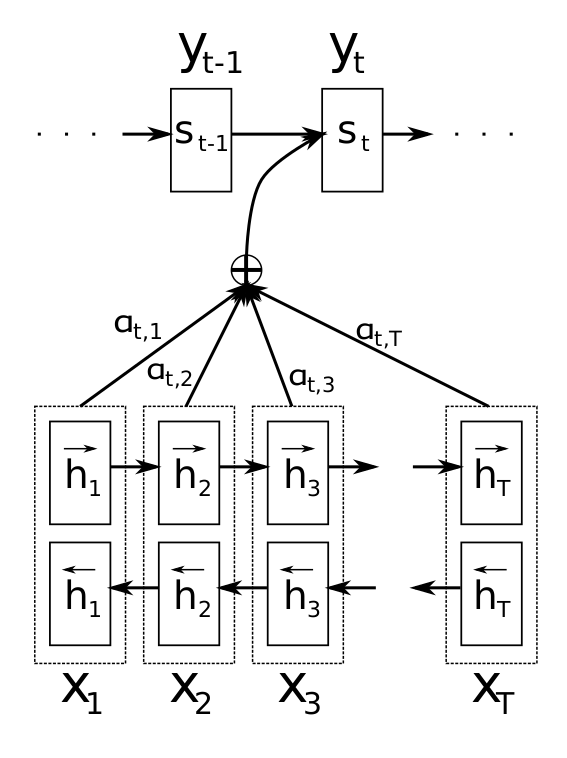
\includegraphics[scale=0.4]{images/attention}
	\caption{Attention based encoder \citep{bahdanau2014neural}}.
	\label{attention}
\end{figure}

\subsection{Unsupervised Morphological induction}

\cite{soricut2015unsupervised} proposed a language-agnostic, heuristic method to capture morphological transformations by exploiting regularities present in word embeddings \citep{mikolov2013distributed}. Their method automatically induces morphological rules and transformations to represent them as vectors in the same embedding space. During testing, out of vocabulary words can be mapped into the same vector space using the learned morphological transformations. In this algorithm, the morphological rules are learned as follows.

\begin{enumerate}
	\item Extract candidate morphological rules like \textit{('suffix', 'ies', 'y')} (replace suffix \textit{ies} with \textit{y}) from word pairs in vocabulary V and evaluate their quality in the pre-trained embedding space.
	\item Generate morphological transformation from the above candidate rules and build a cyclic, multi-graph representing words as nodes and edges as morphological transformations.
	\item Build a normalized acyclic graph (based on word frequency) with 1-1 morphological mapping from the above graph.
	\item Map the rare/out of vocabulary words in the same vector space using morphological transformation using the graph.
\end{enumerate}

Using this approach, if the word \textit{unassertiveness} occurs in the source sentence and is not found the vocabulary of the word embedding, we would be able to get a reasonably good vector representation for the word. Traditionally, any word not in vocabulary is mapped to \textit{unk}. Using the approach from  \cite{soricut2015unsupervised}, we will be able to learn vector representation for morphological transformations like \textit{(prefix,un,$\epsilon$)} and \textit{(suffix,$\epsilon$,ness)}. Then, these morphological rules and their vector representation can be used to map the OOV word \textit{unassertiveness} to  \textit{assertive} and get a good vector representation. 




\chapter{Vector Representations for OOV words}
\label{comparision1}
%In the last chapter, we discussed why it is important to get
In this chapter, we compare different approaches to generate vector representations for OOV words. \citeauthor{soricut2015unsupervised}'s approach is implemented and compared with other existing approaches. The goal of this study is to compare various techniques and use the best performing model in NMT. The models reported in this study are not specific to machine translation. However, they are general methods used to generate vector representations for any word based on its morphology, or the subword units present in them. 

In this experiment, we compare the performance of three popular pre-trained word embeddings models \citep{mikolov2013distributed,pennington2014glove,bojanowski2016enriching} and the implemented morphological transformation approach on standard word similarity dataset. We try to answer the following questions through this study.

\begin{itemize}
	\item What are all the techniques to generate a vector representation for OOV words and their performance? 
	\item How does the implemented morphological transformation technique compare against other approaches?
	\item Which technique would be ideal to use in NMT systems for handling OOV words?
%	\item Which techniques generates the most accurate vector representation for these words?

\end{itemize}


%\section[Section Title. Section Subtitle]{Experiment 1:\\ {\large A Comparison of Vector Representation for OOV words}}

\section{Dataset and Evaluation Metric}

We use the Stanford \textbf{Rare Word (RW) Similarity dataset}  for English from \cite{luong2013better} to evaluate the vector representation of rare words. This dataset contains 2034 morphologically complex word pairs with similarity scores for each pair. They used Amazon mechanical turk to collect 10 human similarity rating on a scale of 0 to 10 for each word pair. The average of all the human judgement scores is taken as the similarity score. The words in RW dataset have a higher degree of English morphology compared to other word-similarity datasets. So, an evaluation on this dataset can be used as a measure of the ability to handle rare and unknown words.

To study the performance, we use \textbf{Spearman's rank correlation coefficient} $\rho$ \citep{spearman1904proof}. The value varies from 0 to 1, with 1 indicating perfect correlation. We use it to report the correlation of the cosine similarity values between the word vectors for each pair, and the human judgement scores.

\section{Results}

The performance of all the models on RW dataset is presented in Table \ref{rw_results}. For skipgram \citep{mikolov2013distributed} and GloVe \citep{pennington2014glove} models, we used the publicly available pre-trained word embeddings. On top of skipgram vectors and GloVe vectors, we induce morphological transformations and report their performance. For both the fastText model, we use their pre-trained model trained on Wikipedia dump\footnote{https://fasttext.cc/docs/en/pretrained-vectors.html}. 

For \textit{fastText + subword} model, we use the pretrained sub-word model from \citep{bojanowski2016enriching} to handle OOV words. We used this instead of \textit{fastText + morph} for two reasons: a) \textit{subword} model can handle any OOV word whereas the \textit{morph} model cannot handle words for which the morphological transformation are not extracted from available words. b) \textit{fastText + subword} model is one best performing model in RW dataset reported in the literature \citep{bojanowski2016enriching}.

\begin{table}[h]
	\centering
	\begin{tabular}{|l|c|c|}
		\hline
		\textbf{Word Embedding Models}                                                                & \textbf{\begin{tabular}[c]{@{}c@{}}Spearman Correlation \\$ \rho \times 100$\end{tabular}}  &
		\textbf{\begin{tabular}[c]{@{}c@{}}No of word pairs handled \\$(2034)$\end{tabular}}  \\ \hline
		SkipGram                                                                              & 22.9          & 1825                                                                                    \\ \hline
		SkipGram + morph                                                           & 24.5 \textbf{(+1.6)}  
		& 1988                                                                                            \\ \hline
		GloVe 6B  & 22.5   &1782                                                                                          \\ \hline
		GloVe 6B + morph             & 25.9                                        \textbf{(+3.4)}       &1996\\ \hline
		fastText    & 29.9   & 1966\\ \hline
		fastText + subword   & 36.76   & 2034\\ \hline
		%\begin{tabular}[c]{@{}l@{}}Bojanowski et al (2016)\end{tabular} & 48                                                                                               \\ \hline
		%Sun et al (2016)                                                                   & 50.4                                                                                               \\ \hline
		%Barkan (2017)                                                                      & 52.5                                                                                               \\ \hline
	\end{tabular}
	\caption{Performance of pre-trained and morphological transformation induced word embeddings on RW dataset}
	\label{rw_results}
\end{table}

From Table \ref{rw_results}, it can be seen that inducing morphological transformations improves the Spearman correlation between human judgement and predicted cosine similarity. By using this method, vector representations for approximately 10\% more words were obtained for SkipGram and GloVe. The high correlation indicates that the vector representations for OOV words (10\%) are almost as good as vector representations for the known words. 
%(1782 words using glove6B and 1996 words using glove6B + Morph). 

%The spearman correlation on RW dataset, for this implementation and other word embeddings models are shown in Table 1.  This is the reason for the huge difference in correlation between models shows in Table \ref{my-label} and Table 2. From Table 2,  


Despite the increase in performance by using morphological transformations, we were not able to map all the OOV words to an in-vocabulary word. We were able to generate word vectors for only 1996 out of 2034. Even the baseline fasttext model from \cite{bojanowski2016enriching} outperforms all the other models by a good margin. When OOV words are handled based on their subword information, we see approximately 7-point increase in the Spearman correlation $\rho$. Also, the \textit{fasttext + subword} model is able to generate vector representation for all the words.  


\section{Implementation challenges}
In our implementation of morphological induction, we were able to improve on the baseline by approximately 2 points. However, we were not able to replicate the results of the original paper. \citeauthor{soricut2015unsupervised} used a  500-dimension skipgram model as their baseline model. They report a 6-point increase in Spearman $\rho$ over their baseline model.  There are a few differences in the implementation from the original model, that may have hindered the algorithm from generating better morphological transformations.

In our implementation, the morphological rules were extracted only from 100,000 most frequent words, from a vocabulary of 3 million words. This was done to allow quick turn around time for implementation and experimentation of the algorithm. Common words are morphologically poorer as compared to rarer words. Extracting morphological rules from all the words in vocabulary may result in further increase in the correlation.

To find the nearest neighbour for a given vector in the vector space, we used a k-d tree based nearest neighbour search. We used 100 trees to build the indexing for all the vectors. This allows for faster querying at the cost of precision. Building the index using more number of trees, say 300, will allow for higher precision at the cost of querying time.


\subsection*{Summary}
From this experiment, we observe that \citeauthor{bojanowski2016enriching}'s approach generates a  semantically more accurate vector representation for words in RW dataset, as compared to other models. The model can also generate accurate word representations for all possible words. This is a very important property that can aid translation for morphologically rich languages. Based on this result, we use the fasttext model in NMT system to handle OOV words which we will discuss in the next chapter.

\chapter{MT for Morphologically Rich Languages}
\label{experiments}
In this chapter, we present how we use the fasttext model to expand source vocabulary and improve the quality of machine translation for morphologically rich languages. In Section \ref{sec:mtdataset}, we describe the dataset used for the translation task. We present the pre-processing steps and training details in Section \ref{preprocess}. In Section \ref{sec:mt_eval}, we describe the evaluation metric used to report the quality of generated translations. The performance of the proposed approach is presented in the Section \ref{sec:du_en} and Section \ref{sec:tr_en}. 

For the proposed approach, the translation task is performed on two language pairs: German $\rightarrow$ English and Turkish $\rightarrow$ English. Both these languages are morphologically rich and well studied in previous works \citep{bahdanau2014neural,luong2015effective,sennrich2015neural,gulcehre2015using}, particularly German - English translation. They also have a very large vocabulary making them ideal candidates for this study. German $\rightarrow$ English is high resource task in machine translation with 4.5M sentence pairs available for training. But, Turkish $\rightarrow$ English is low resource task with around 160,000 sentence pairs available for training. For the experiments in this study, both of the languages are studied under low-resource settings; since the goal of this study is to improve translation performance for morphologically rich, low-resource languages.

%From these experiments, we try to answer the following question

%\begin{itemize}
%	\item 
%\end{itemize}



\section{Dataset }
\label{sec:mtdataset}

%The translation task was performed on two languages: German $\rightarrow$ English and Turkish $\rightarrow$ English. 
For both of the language pairs, we used the WIT$^{3}$ dataset \citep{cettolo2012wit3} from IWSLT'14 machine translation track \citep{cettolo2014report}. The dataset consists of sentence aligned subtitles for TED and TEDx talks. WIT dataset contains 149,000 sentence pairs for Turkish - English and 160,000 sentence pairs for German - English. During testing time, the translation performance is reported on test data from the WIT$^{3}$ corpus. Additionally, German $\rightarrow$ English model will also be evaluated newstest2012 (3000 sentences) and newstest2013 (3000 sentences) dataset from ACL WMT'14. We do this as a measure of generalization, since the newstest data is from a different domain than training data. 

%For testing, we use test data provided in the same WIT$^{3}$ dataset. 

%Our validation set comprises of 6969 sentence pairs which was taken from the training data. The test set is a concatenation of dev2010, dev2012, tst2010, tst2011 and tst2012 which results in 6750 sentence pairs. The English dictionary has 22822 words while the German has 32009 words.


\begin{table}[!htb]
	\begin{subtable}{.5\linewidth}
		\centering
		
		\begin{tabular}{|l|l|l|}
			\hline
			& Turkish     & English     \\ \hline
			No. of sentences         & \multicolumn{2}{c|}{149k} \\ \hline
			No. of words             & 3.3M        & 2.7M        \\ \hline
			Unique words      & 160k         & 48k         \\ \hline
%			Average  Length & 31.6        & 22.6        \\ \hline
		\end{tabular}
		\caption{Turkish - English}
	\end{subtable}%
	\begin{subtable}{.5\linewidth}
		\centering
		
		\begin{tabular}{|l|l|l|}
			\hline
			& German     & English     \\ \hline
			No. of sentences         & \multicolumn{2}{c|}{160k} \\ \hline
			No. of words             & 3M        & 3.1M        \\ \hline
			Unique words      & 112k         & 49k         \\ \hline
%			Average  Length & 18.5       & 17.5       \\ \hline
		\end{tabular}
		\caption{German - English}
	\end{subtable}
	\caption{Training data statistics} 
	\label{stats}
\end{table}

In addition to above datasets, we used the pre-trained word embedding model\footnote{https://fasttext.cc/docs/en/pretrained-vectors.html} from \cite{bojanowski2016enriching} for English, German and Turkish. These word vectors are trained on Wikipedia data \footnote{https://dumps.wikimedia.org/}. 


\section{Training}
\label{preprocess}
The data was preprocessed using a data preparation script\footnote{https://github.com/facebookresearch/MIXER/blob/master/prepareData.sh} from \cite{ranzato2015sequence}. The Moses tokenizer is used to tokenize the sentences. All sentences are converted to lowercase and sentences with more than 80 words are removed. Detailed statistics of the parallel corpora used for training is given in Table \ref{stats}. The source and target vocab size was limited to 50k for training.
 
In all our models, the embedding layer dimension is 300. The number hidden layers in encoder and decoder is set to 2, each layer with 500 dimensions. We trained all our models for 20 epochs, using Adam optimizer and used the best performing model based on accuracy and perplexity for evaluation. The batch size was fixed to 128. As suggested \cite{luong2015effective}, we use a dropout probability of 0.2 for our LSTMs. We trained our models on Nvidia Tesla P100 GPU, from Compute Canada\footnote{www.computecanada.ca}, where we achieved a speed of 5k target words per second.  


%\begin{table}[!htb]
%	\caption{Statistics of Training Data}
%	\begin{minipage}{.5\linewidth}
%		\caption{Turkish-English}
%		\centering
%		
%	\end{minipage}
%	\begin{minipage}{.5\linewidth}
%		\centering
%		\caption{German-English}
%		\begin{tabular}{|l|l|l|}
%			\hline
%			& Turkish     & English     \\ \hline
%			Sentences         & \multicolumn{2}{c|}{160k} \\ \hline
%			Words             & 3.3M        & 2.7M        \\ \hline
%			Unique words      & 160         & 48k         \\ \hline
%			Average  Length & 31.6        & 22.6        \\ \hline
%		\end{tabular}
%	\end{minipage} 
%\end{table}
%Additionally, for turkish I used the SETimes corpus
%
%For the experiment on vocasflakfds, I used pre-trained word embeddings from \cite{mikolov2013efficient,mikolov2013distributed}, \cite{pennington2014glove} and \cite{bojanowski2016enriching}. In their work, the authors used words vectors of 500 dimensions. In this experiment, I used embeddings of size 300 dimensions for SGNG and 50 dimensions for Glove.  

%The proposed approach will be evaluated on English-German translation using the bilingual, parallel corpora from ACL WMT 2016\footnote{http://www.statmt.org/wmt16/translation-task.html}. The training corpora include Europarl (1.9M sentences), Common Crawl corpus (2.3M sentences) and News Commentary v11 (240,000 sentences). newstest2013 (3000 sentences) and newstest2014 (3000 sentences) data will be used as validation dataset.

\section{Evaluation}
\label{sec:mt_eval}
To be comparable with other existing NMT systems, we have evaluated the models using standard BLEU score metric from  \cite{papineni2002bleu}. BLEU is one of the most popular and widely used automatic MT evaluation metric. The score varies from 0 to 100 and higher scores denote better translation. It reports the correlation of machine translations with human translations measured using the degree of n-gram overlap. As a baseline model, the attention model from \cite{luong2015effective} was used. Then, the proposed OOV word handling approach will be added to the baseline model, and the translation performance will be studied. 

During the testing time, the vocabulary of the proposed model is expanded dynamically. To do this, we first create a vocabulary of all the words in the source language sentences. For each word in the vocabulary, we use pre-trained embedding model from \cite{bojanowski2016enriching} to generate vector representation. In this model, each word $w$ is represented as bag of character $n$-grams. For example, the word \textit{where} will be represented using character $n$-grams \textit{ $<$wh, whe, her, ere, re$>$ } and the special sequence \textit{$<$where$>$}. The vector representation of the word $w$ is the sum of vector representations of its $n$-grams. Mathematically, this can be defined as follows:

\begin{equation}
s(w,c) = \sum_{g \in G_w} z_g^{T} v_c.
\end{equation}

where $w$ is the input word and $c$ is the context word. $z_g$ and $v_c$ are the vector representations for each $n$-gram and context word respectively. $G_w$ is the set of all $n$-grams appearing in the word $w$. Then, the embedding matrix of the NMT system is concatenated with the vector representations the OOV words obtained using the above model.

%If the proposed model shows an improvement in BLEU score, this work can be extended and applied to languages with richer morphology, especially agglutinative languages like Turkish or Tamil.



%First, do words embeddings trained from machine translation hold similar properties as word embeddings trained for language modelling. 
%No, they do not hold the same properties.

%
%\begin{table}[]
%	\centering
%	\begin{tabular}{|l|l|l|}
%		\hline
%		\multicolumn{1}{|c|}{\textbf{System}}                                                   & \multicolumn{2}{c|}{\textbf{BLEU}} \\ \hline
%		& tedtest       & newstest2013       \\ \hline
%		Global Attention Model                                                                  & 27.58         & 13.73              \\ \hline
%		\begin{tabular}[c]{@{}l@{}}Global Attention Model\\ + vocabulary expansion\end{tabular} & 28.20         & 15.01              \\ \hline
%	\end{tabular}
%	\caption{German $\rightarrow $ English Translation performance on IWSLT test set and newstest2013.}
%	\label{my-label}
%\end{table}


\section{German $\rightarrow$ English Translation}
\label{sec:du_en}
Table \ref{german_results_indomain} and Table \ref{german_results_outdomain} present comparisons of proposed approach with the baseline model from \cite{luong2015effective} on German $\rightarrow$ English translation. The results demonstrate that the proposed vocabulary expansion significantly improves the translation performance, particularly for out of domain data. The performance gain is noted separately for adding fixed word embedding and for adding expanded vocabulary. 

As reported in Table \ref{german_results_indomain}, for in-domain test data, the performance gains for the proposed approach are in the range of approximately 2-2.8 BLEU points. As a measure of generalization, we also studied the performance on out of domain data. On the test data from WMT'14, the performance gains are approximately 3 BLEU points. We notice that the performance gain is higher in out of domain data, making this approach very suitable for low resource languages. 

\begin{table}[ht]
	\centering
	\begin{tabular}{|l|l|l|l|}
		\hline
		\multicolumn{1}{|c|}{\textbf{System}}                                                                                  & \multicolumn{3}{c|}{\textbf{\begin{tabular}[c]{@{}c@{}}BLEU score on \\ IWSLT test data \end{tabular}}} \\ \hline
		& tst2010                       & tst2011                         & tst2012                      \\ \hline
		Global Attention Model                                                                                                 & 27.09 $\pm$ 0.96   &
		30.32 $\pm$ 0.97      &    
		27.11 $\pm$ 0.91                   \\ \hline
		\begin{tabular}[c]{@{}l@{}}Global Attention Model\\ + pre-trained word embeddings\end{tabular}                          & 27.40   $\pm$ 0.95                      & 
		31.25   $\pm$ 0.99                        &
		26.80   $\pm$ 0.89           \\ \hline
		\begin{tabular}[c]{@{}l@{}}Global Attention Model\\ + pre-trained word embeddings \\ + expanded vocabulary\end{tabular} & 
		\textbf{29.04  $\pm$ 0.90}                       &
		\textbf{33.18  $\pm$ 1.03}                         &
		\textbf{28.23  $\pm$ 0.88}                      \\ \hline
		
	\end{tabular}
	\caption{German $\rightarrow $ English Translation performance on \textbf{in-domain test data} from IWSLT'14 with 95\% confidence interval}
	\label{german_results_indomain}
\end{table}


\begin{table}[ht]
	\centering
	\begin{tabular}{|l|l|l|}
		\hline
		\multicolumn{1}{|c|}{\textbf{System}}                                                                                  & \multicolumn{2}{c|}{\textbf{\begin{tabular}[c]{@{}c@{}}BLEU on \\ WMT test data\end{tabular}}} \\ \hline
		& news2012                                      & news2013                                       \\ \hline
		Global Attention Model                                                                                                 & 10.85  $\pm$ 0.37                                   & 13.09 $\pm$ 0.43                                  \\ \hline
		\begin{tabular}[c]{@{}l@{}}Global Attention Model\\ + pre-trained word embeddings\end{tabular}                          &
		12.75 $\pm$ 0.44                                         &
		14.67  $\pm$  0.44                                       \\ \hline
		\begin{tabular}[c]{@{}l@{}}Global Attention Model\\ + pre-trained word embeddings \\ + expanded vocabulary\end{tabular} &
		\textbf{13.77 $\pm$ 0.45}                                       & \textbf{16.01  $\pm$ 0.5}                                         \\ \hline
	\end{tabular}
	\caption{German $\rightarrow $ English Translation performance on \textbf{Out of domain test data} from WMT'14 with 95\% confidence interval}
	\label{german_results_outdomain}
		
\end{table}

%\begin{table}[ht]
%	\centering
%	\begin{tabular}{|c|c|c|c|c|c|}
%		\hline
%		\multicolumn{1}{|c|}{\textbf{System}}                                                                                  & \multicolumn{5}{c|}{\textbf{BLEU}}                                            \\ \hline
%		\multicolumn{1}{|c|}{\multirow{2}{*}{}}                                                                                & \multicolumn{3}{c|}{In domain data (IWSLT)} & \multicolumn{2}{c|}{Out of domain data (WMT)} \\ \cline{2-6} 
%		\multicolumn{1}{|c|}{}                                                                                                 & tst2010    & tst2011    & tst2012   & newstest2012       & newstest2012       \\ \hline
%		Global Attention Model                                                                                                 & 27.07 $\pm$ 0.96      & 30.34 $\pm$ 0.96     & 27.12  $\pm$ 0.96   & 10.86  $\pm$ 0.96            & 13.10              \\ \hline
%		\begin{tabular}[c]{@{}l@{}}Global Attention Model\\ + fixed word embeddings\end{tabular}                          & 27.44      & 31.23      & 26.78     & 12.77              & 14.68              \\ \hline
%		\begin{tabular}[c]{@{}l@{}}Global Attention Model\\ + fixed word embeddings \\ + expanded vocabulary\end{tabular} &    29.04        &  33.17          &  28.20         &      13.77              &     16.02               \\ \hline
%	\end{tabular}
%	\caption{German $\rightarrow $ English Translation performance on IWSLT test data and newstest data.}
%	\label{german_results}
%\end{table}



Two possible explanations for the huge performance gap between in-domain data and out of domain data are:
\begin{itemize}
	\item The model was trained in spoken language domain from IWSLT. However, the test data from WMT is news data (written language). Written languages are generally more complicated than spoken languages.
	\item Out of Vocabulary words (both source and target) are higher in WMT test data in comparision to IWSLT test data.
\end{itemize}

It has already been shown in the literature that using pre-trained word embedding helps in faster convergence and improved performance \citep{garcia2015document,delbrouck2017visually}. This is shown in the small increase of the BLEU score in the second column of the Table \ref{german_results_indomain} and Table \ref{german_results_outdomain}. By fixing the word representations, we retain the linguistics properties captured in the word embedding model. This helps in translating OOV words.

In the \textit{Global attention model} and \textit{Global attention model + fixed word embeddings}, the vocabulary size of the network is fixed at 50,000. When using the expanded vocabulary model, the vector representations for all the unknown words are generated using fastText \citep{bojanowski2016enriching}. Because of this, the out of vocabulary words which are semantically similar or morphologically related to an in-vocabulary word gets translated correctly. In the literature, we found only \cite{bahar2017rwth} reported performance on the same test data as ours. They reported a performance of 37.3 BLEU points on tst2010. The difference in performance of their model and our model can be attributed to the size of training data. They used 2.1M parallel sentence pairs for training while we used only 160k.

%Also, the morphological and semantic regularities preent in the word embedding model are also used map OOV words.




\section{Turkish $\rightarrow$ English Translation}
\label{sec:tr_en}
To study the suitability of the approach to a morphologically more complex but low resource language, we ran the experiments on Turkish $\rightarrow$ English translation. Table \ref{turkish_results} presents the performance of the proposed approach and the baseline attention model. The results demonstrate that the translation performance significantly improved compared to the baseline attention model. We report performance only on in-domain data from IWSLT'14. To the best of my knowledge, no other test dataset is available to test the out of domain performance.

Similar to German $\rightarrow$ English, when we use pre-trained word embeddings alone, the performance improves by 1.0 - 1.5 BLEU points. The source vocabulary expansion technique gives another 1.2 BLEU points improvement. Overall, we achieve performance gain of 1.6 - 2.3 BLEU points by expanding the vocabulary of the source language.

\begin{table}[ht]
	\centering
	\begin{tabular}{|l|l|l|l|}
		\hline
		\multicolumn{1}{|c|}{\textbf{System}}                                                                                  & \multicolumn{3}{c|}{\textbf{BLEU}} \\ \hline
		& tst2010    & tst2011   & tst2012   \\ \hline
		Global Attention Model                                                                                                 & 15.60 $\pm$ 0.72     & 15.79 $\pm$ 0.83    & 16.02 $\pm$ 0.73    \\ \hline
		\begin{tabular}[c]{@{}l@{}}Global Attention Model\\ + pre-trained word embeddings\end{tabular}                          & 16.16 $\pm$ 0.72     & 17.11  $\pm$ 0.86    & 17.27 $\pm$ 0.75    \\ \hline
		\begin{tabular}[c]{@{}l@{}}Global Attention Model\\ + pre-trained word embeddings \\ + expanded\end{tabular} & \textbf{17.21 $\pm$ 0.75}     & \textbf{18.31 $\pm$ 0.90 }    & \textbf{18.41 $\pm$ 0.75}   \\ \hline
	\end{tabular}
	\caption{BLEU Score: Turkish $\rightarrow$ English on IWSLT'14 data}
	\label{turkish_results}
\end{table}

The difference in performance between German $\rightarrow$ English and Turkish $\rightarrow$ English can be attributed to the low resource availability of Turkish.

\begin{itemize}
	\item The source vocabulary size for German is 110,000 whereas the source vocabulary size for Turkish is 160,000. This makes it harder for the baseline model to capture learn the input-output mapping.
	\item When compared with German $\rightarrow$ English, the low performance of \textit{baseline + pre-trained word vector} and \textit{expanded vocabulary} model can be attributed to the lower quality of the pre-trained word vector for Turkish. The word vector for German was trained on 2.2 million Wikipedia articles whereas the Turkish word vectors were trained on only 100,000 Wikipedia articles.
\end{itemize}



\subsection*{Transformer model}
This vocabulary expansion technique is independent of any underlying architecture. We can use this technique for any word based NMT systems. To study the effectiveness to the vocabulary expansion technique using a different word based NMT system, we ran the same experiment on the transformer model proposed in \cite{vaswani2017attention}. For all the transformer model, we used the same parameters as the original paper. The word vector and RNN size was set to 512 with 6 layers. Adam optimizer with a learning rate of 2 and learning rate decay was used. The result of the experiments are shown in Table \ref{turkish_trans_results}. 

\begin{table}[ht]
	\centering
	\begin{tabular}{|l|l|l|l|}
		\hline
		\multicolumn{1}{|c|}{\textbf{System}}                                                                                  & \multicolumn{3}{c|}{\textbf{BLEU}} \\ \hline
		& tst2010    & tst2011   & tst2012   \\ \hline
		Transformer                                                                                                 & 12.66 $\pm$ 0.66     & 13.51 $\pm$ 0.75    & 13.27 $\pm$ 0.66    \\ \hline
		\begin{tabular}[c]{@{}l@{}}Transformer\\ + pre-trained word embeddings\end{tabular}                          & 17.03 $\pm$ 0.86     & 18.08  $\pm$ 0.86    & 18.86 $\pm$ 0.77    \\ \hline
		\begin{tabular}[c]{@{}l@{}}Transformer\\ + pre-trained word embeddings \\ + expanded vocabulary\end{tabular} & \textbf{18.58 $\pm$ 0.79}     & \textbf{19.76 $\pm$ 0.92}     & \textbf{20.27 $\pm$ 0.80}   \\ \hline
	\end{tabular}
	\caption{BLEU Score: Turkish $\rightarrow$ English on IWSLT'14 data}
	\label{turkish_trans_results}
\end{table}

Compared to the baseline transformer model, we see a significant increase of approximately 4-5 BLEU points when we used pre-trained word embeddings from fasttext. The vocabulary expansion technique further increases the performance by approximately 1.5 BLEU points. 

In the literature, we find that only \cite{sennrich2016improving} and \cite{gulcehre2015using} reported results on the same test data as ours. In both the papers, they used twice the amount of training data as we did. \cite{gulcehre2015using} integrated language model training on monolingual data into an NMT system. \cite{sennrich2016improving} proposed a technique to improve the performance of NMT by constructing synthetic training data obtained using back-translation. \cite{sennrich2016improving} reported a  performance of 21.2 and 21.1 BLEU points on \textit{tst2011} and \textit{tst2012} respectively. We found that the performance of our model and \citeauthor{gulcehre2015using} are very close in \textit{tst2011} and \textit{tst2012}. But \citeauthor{sennrich2016improving}'s model outperforms our model only by approximately 1 BLEU points despite being trained on twice the amount of training data.


\begin{table}[htb!]
	\centering
	\begin{tabular}{|l|l|l|l|l|l|}
		\hline
		& \multicolumn{5}{c|}{BLEU}                                                     \\ \hline
		\multicolumn{1}{|c|}{Dataset}                                                                                           & tst2010 & tst2011 & tst2012 & news2012               & news2013               \\ \hline
		\multicolumn{6}{|c|}{German $\rightarrow$ English}                                                                                                                                                                    \\ \hline
		\begin{tabular}[c]{@{}l@{}}Global Attention Model\\ + pre-trained word embeddings \\ + expanded vocabulary\end{tabular} & 29.04   & 33.18   & 28.23   & \textbf{13.77}                  & \textbf{16.01}                  \\ \hline
		\begin{tabular}[c]{@{}l@{}}Global Attention Model \\ + BPE\end{tabular}                                                 & \textbf{29.78}   & \textbf{34.23 }  & \textbf{30.17}   & 4.78                   & 5.32                   \\ \hline
		\multicolumn{6}{|c|}{Turkish $\rightarrow$ English}                                                                                                                                                                   \\ \hline
		\begin{tabular}[c]{@{}l@{}}Transformer \\ + pre-trained word embeddings \\ + expanded vocabulary\end{tabular}           & 18.58   & 19.76   & \textbf{20.27}   & \multicolumn{1}{c|}{-} & \multicolumn{1}{c|}{-} \\ \hline
		\begin{tabular}[c]{@{}l@{}}Transformer\\ + BPE\end{tabular}                                                             & \textbf{19.04}   & \textbf{20.46 }  & 20.00   & \multicolumn{1}{c|}{-} & \multicolumn{1}{c|}{-} \\ \hline
	\end{tabular}
	
	\caption{Comparision with BPE for both the language pairs}
	\label{comparision}
\end{table}

\section{Comparison with BPE}
In this section, we compare the source vocabulary expansion approach with BPE approach proposed in \cite{sennrich2015neural}. BPE is particularly useful for morphologically rich language as it operates at subword level and capable of modeling open-vocabulary translation. Table \ref{comparision} presents the performance of both the models when trained on IWSLT'14 dataset. 

In in-domain data, BPE approach consistently outperforms our approach by approximately 0.5 - 1 BLEU points. For both the language pairs, BPE encoding reduced the source vocabulary approximately 7k - 8k ad target vocabulary to approximately 5k resulting in faster training time. But for out-of-domain data, BPE performed very poorly in comparison to our model. We suspect that the BPE code learned on IWSLT dataset did not fit the test data from newstest. In Table \ref{sample_trans}, we present some of translations from the baseline models and the vocabulary expanded model. 
\begin{table*}%[tbh!]
	\centering
	\resizebox{15cm}{!}{
		\begin{tabular}{|c|c|p{15.5cm}|}
			% sent 1046 
			\hline
			\hline
			\multirow{7}{*}{1} & \textit{Source} & sie wuchs zu einer zeit auf , in der konfuzianismus die soziale norm und der lokale mandarin die wichtigste person war. \\
			& \textit{Target} & she grew up at a time when confucianism was the social norm and the local mandarin was the person who mattered. \\
			\cline{2-3}
			& \multirow{2}{*}{\it{Baseline}} & it grew up at a time when the social norm and the social norm was the most important person in retirement.\\
			\cline{2-3}
			& \it{+ fixed embedding} & she grew up at a time when the social norm and the local chinese , the most important person was . \\
			\cline{2-3}
			& \multirow{2}{*}{\it{+ expanded vocab}} & she grew up at a time in buddhism , the social norm , and the local speaker was the most important person .\\
			\hline
			\hline
			% sent 80
			\multirow{7}{*}{2} & \textit{Source} & evolution bedeutet nicht zwangsläufig das längste leben zu bevorzugen.\\
			& \textit{Target} & evolution does not necessarily favor the longest-lived. \\
			\cline{2-3}
			& \multirow{1}{*}{\it{Baseline}} & evolution doesn't necessarily mean the longest biggest life. \\
			\cline{2-3}
			& \it{+ fixed embedding} & evolution doesn't necessarily mean the longest life to prefer. \\
			\cline{2-3}
			& \multirow{1}{*}{\it{+ expanded vocab}} & evolution doesn't necessarily mean to prefer the longest life .\\
			\hline
			\hline
			
		\end{tabular}
	}
	\caption{\textbf{Sample translations - }for each example, the source sentence, target translation, baseline translations and vocabulary expanded translation are showed.}
	\label{sample_trans}
\end{table*}

\subsection*{Summary}
In this chapter, we presented an experimental evaluation of how the quality of machine translation for morphologically rich languages can be improved by expanding source language vocabulary. We achieve a performance gain of 2-3 BLEU points for both German $\rightarrow$ English and Turkish $\rightarrow$ English. We also note that we see a larger performance gain on out of domain data as compared to in-domain data. We also compared the performance with another popular approach for morphologically rich languages. Our model is competitive, but doesn't outperform BPE in in-domain data. In out-of-domain data, our model performs better than BPE. 

%\subsection{Vocabulary Expansion}
%\begin{itemize}
%	\item Train word embeddings using language modelling
%	\item Use 50k most frequents word in word embeddings in NMT without updating
%	\item For rare and unknown words, do a morphological analysis to get more accurate word representations.	
%\end{itemize}

%
%\begin{table}[]
%	\centering
%	\begin{tabular}{|l|l|l|}
%		\hline
%		\multicolumn{1}{|c|}{\textbf{System}}                                                   & \multicolumn{2}{c|}{\textbf{BLEU}} \\ \hline
%		& tedtest       & newstest2013       \\ \hline
%		Global Attention Model                                                                  & 27.58         & 13.73              \\ \hline
%		\begin{tabular}[c]{@{}l@{}}Global Attention Model\\ + vocabulary expansion\end{tabular} & 28.20         & 15.01              \\ \hline
%	\end{tabular}
%	\caption{Turkish $\rightarrow $ English Translation performance on IWSLT test set and newstest2013.}
%	\label{my-label}
%\end{table}


\chapter{Conclusion and Future Work}
\label{conclusion}


\section{Summary}
Machine translation can aid in overcoming the human language barrier in communication. Current translation systems rely on large amounts of parallel corpora for training. But, most of the languages in the world have only a very small amount data available for training these system. Translating morphologically rich languages is more difficult as compared to morphologically poor languages. 


In this project, our goal was to improve the quality of machine translation for morphologically rich, low-resource languages. We presented a vocabulary expansion technique that improved the machine translation from (German and Turkish) $\rightarrow$ English. We demonstrated that our approach improved the translation performance by approximately 2-3 BLEU points.

In our proposed approach, we use pre-trained, fixed word vectors as our input. By doing so, we separated the problem of handling Out of Vocabulary (OOV) words from NMT systems. Therefore, as long as the word embeddings capture the morphological and semantic information of the words and exhibit regularity in their mapping, the translation systems will be able to use that information to translate OOV words. 

Our approach is independent of the underlying architecture of the base NMT system. This technique can be incorporated in any NMT systems that work at word level instead of character or sub-word level.

\section{Future Directions}

In our approach, we used a simple attention based NMT system from \cite{luong2015effective}, as the underlying base system. The performance in the translation task is limited by the ability of the base system. In future, more experiments, with varying training data sizes can be done on more sophisticated models like purely attention based architecture or convolution neural network (CNN) can be done. Recently, \cite{gehring2017convolutional} proposed a fully parallelizable CNN architecture for translation. \cite{vaswani2017attention} proposed a simple network architecture without using any recurrence or convolution. These two networks can be a very good candidate for a base system.


Another promising direction to explore is the expansion of target vocabulary of NMT systems. If a similar improvement is observed in the translation quality, the training time of the network can be greatly reduced.

%\section{Implementation status and Timeline}

The current status of the project and an estimated timeline for my proposed work has been given in the table \ref{timeline}.

\begin{table}[!htbp]
	\centering
	\resizebox{\textwidth}{!}{%
		\begin{tabular}{|l|c|}
			\hline
			\textbf{Work}                                                                                                                             & \textbf{Expected completion date} \\ \hline
			Proposal defense                                                                                                                          & Feb, 2018                        \\ \hline
			\begin{tabular}[c]{@{}l@{}}Implementation of morphological analyzer \\ \citep{soricut2015unsupervised}               \end{tabular}                                                                                                            & Completed                        \\ \hline
			\begin{tabular}[c]{@{}l@{}}Implementation of NMT system \\ \citep{bahdanau2014neural} \end{tabular}                                                                                       & Completed                      \\ \hline
			Handling OOV in NMT                                                                                                                           & In progress                         \\ \hline
			Result analysis  and report writing                                                                                                                          & Feb - Mar, 2018                         \\ \hline
		\end{tabular}%
	}
	\caption{Thesis Timeline}
	\label{timeline}
\end{table}


\newpage
\appendix
\chapter{List of Abbreviations and Definitions}

\begin{description}[leftmargin=!,labelwidth=\widthof{\bfseries The longest label}]
	\item[BLEU] Bilingual Evaluation Understudy
	\item[BPE] Byte Pair Encoding
	\item[CNN] Convolution Neural Network
	\item[GRU] Gated Recurrent Unit
	\item[LSTM] Long Short-Term Memory
	\item[MT] Machine Translation
	\item[NMT] Neural Machine Translation
	\item[OOV]  Out Of Vocabulary words
	\item[RNN] Recurrent Neural Network
	\item[SMT] Statistical Machine Translation
	\item[Morpheme] The smallest meaningful units in a language.
	\item[Word embedding] A technique used to map and represent words in a language as vectors of real number, where words with similar meaning have similar representations.
	\item[Word vector] A vector used to represent a word in the vector space. Also known as \textit{Word representations}
	\item[Morphological rich languages] Languages that encode large amount of information through morphology. They have a very large vocabulary size since there can large number of word forms per lexeme.
\end{description}


% SUmmarize key points. less emphasis on technical grounds. Put in exact technical content.

\bibliography{bib}
\bibliographystyle{apalike}


\end{document}
